\chapter{Results}
All of the recorded data that is presented in the following sections can also be found in the project spreadsheet on Google Sheets~\cite{projectSpreadsheet}. 

\section{Overview of Search Space}
\begin{figure}[tbph]
    \centering
    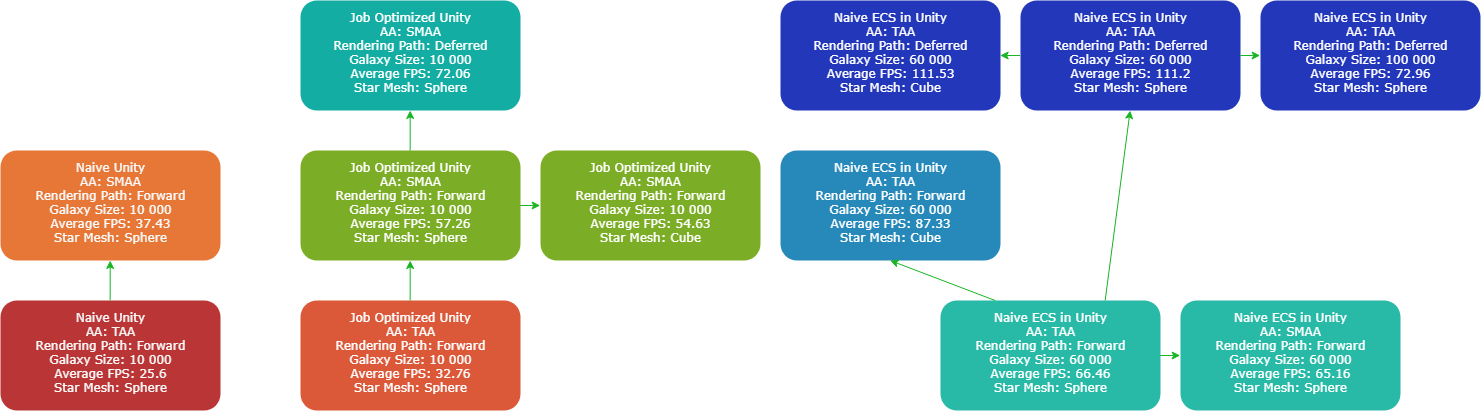
\includegraphics[width=1\textwidth]{Figures/SearchSpace.png}
    \caption[Optimisation Search Space And Combinations]{The space of optimisations that were measured}
    \label{fig:searchspace}
\end{figure}

In terms of the search space for testing, there are a large variety of possible optimisations. Given the time and scope of the project, it is not feasible to measure everything that springs to mind. The full search space and the combination of optimisations that I worked with can be found in Figure~\ref{fig:searchspace}.

\section{Frame Latency Results}
In terms of frame latency, lower values mean higher performance as frames are delivered more quickly. The order of the legend in the following latency graphs is relative to the order which these conditions were tested. This means that the top one is the first test and the bottom one is the last test in each graph. Test results also make use of the forward rendering path by default. 

\subsection{Naive Unity Tests}
\begin{figure}[!p]
    \centering
    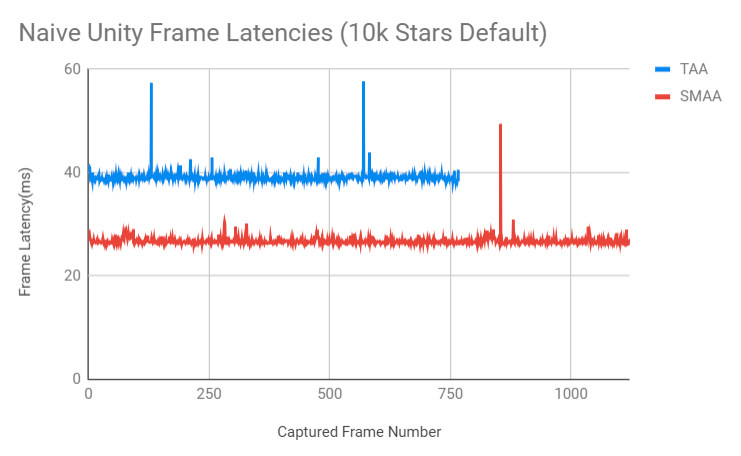
\includegraphics[width=1\textwidth]{Figures/naiveUnityLatencies.png}
    \caption[Combined Frame Latency Chart for Naive Unity Tests]{The combined chart of measured frame latencies for all naive Unity tests}
    \label{fig:naiveUnityLatency}
\end{figure}

For the Naive Unity condition, two tests related to anti-aliasing were conducted. The results for this condition can be found in Figure~\ref{fig:naiveUnityLatency}. The results show that opting for SMAA as the method of anti-aliasing yielded the best performance. A video showing off a galaxy using SMAA can be found here~\cite{naiveUnityVideo}. 

\subsection{Job Optimised Unity Tests}
\begin{figure}[!p]
    \centering
    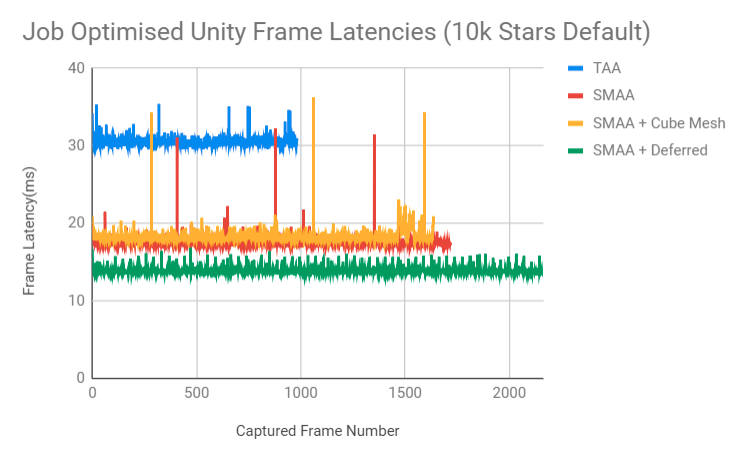
\includegraphics[width=1\textwidth]{Figures/jobOptimisedUnityLatencies.png}
    \caption[Combined Frame Latency Chart for Job Optimised Unity Tests]{The combined chart of measured frame latencies for all job optimised Unity tests}
    \label{fig:jobOptimisedUnityLatency}
\end{figure}

The Job Optimised Unity condition consisted of four different tests. This includes tests for anti-aliasing, mesh complexity and rendering paths. The results for this condition can be seen in Figure~\ref{fig:jobOptimisedUnityLatency}. Similarly to the Naive Unity condition, opting for SMAA instead of TAA improved performance by a decent amount. Using simpler cube meshes did not appear to change the results in any major way. Finally, making use SMAA with the deferred rendering path yielded the best performance. As a bonus, the use of deferred rendering also improved overall stability. A video showing off the SMAA test can be found here~\cite{jobOptimisedUnityVideo}. 

\subsection{Naive ECS Tests}
\begin{figure}[!p]
    \centering
    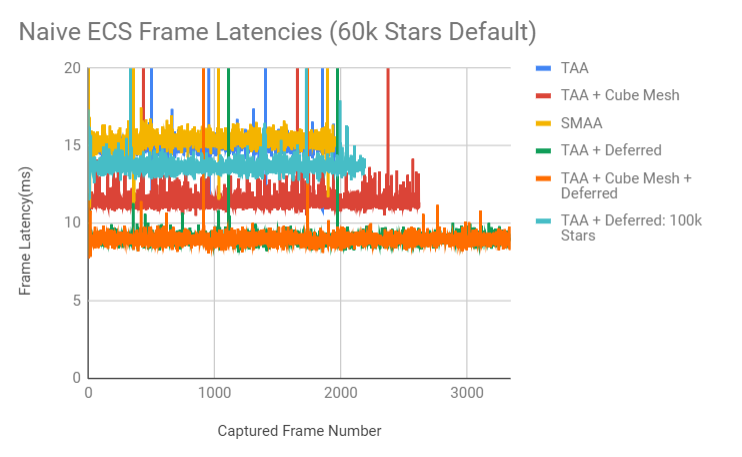
\includegraphics[width=1\textwidth]{Figures/naiveEcsLatencies.png}
    \caption[Combined Frame Latency Chart for Unity Tests]{The combined chart of measured frame latencies for all Naive ECS tests}
    \label{fig:naiveEcsUnityLatency}
\end{figure}

For the Naive ECS condition, a large variety of tests were done. These can be seen in Figure~\ref{fig:naiveEcsUnityLatency}. One thing to keep in mind is that for this condition is that the galaxy had a default size of 60 000 stars in order to properly tax the hardware. A final test case making use of 100 000 stars is also included to provide some insight into the scalability of the best recorded combination of optimisations. 
The graph in this case has limited the maximum y-value for the sake of presentation. 

The results point towards some differences in variables that affect performance. TAA and SMAA usage provide very similar performance while simple cube meshes provided a substantial performance improvement. Similarly to the previous two test conditions, using deferred rendering resulted in the best performance. While using deferred rendering, cube meshes no longer provided any noticeable performance increases. A video demonstrating the TAA test can be found here~\cite{naiveECSVideo} while a video demonstrating the TAA + Deferred with 100 000 stars test can be found here~\cite{naiveECSVideo100k}.

\section{Average Framerate for All Tests}
\begin{figure}[!p]
    \centering
    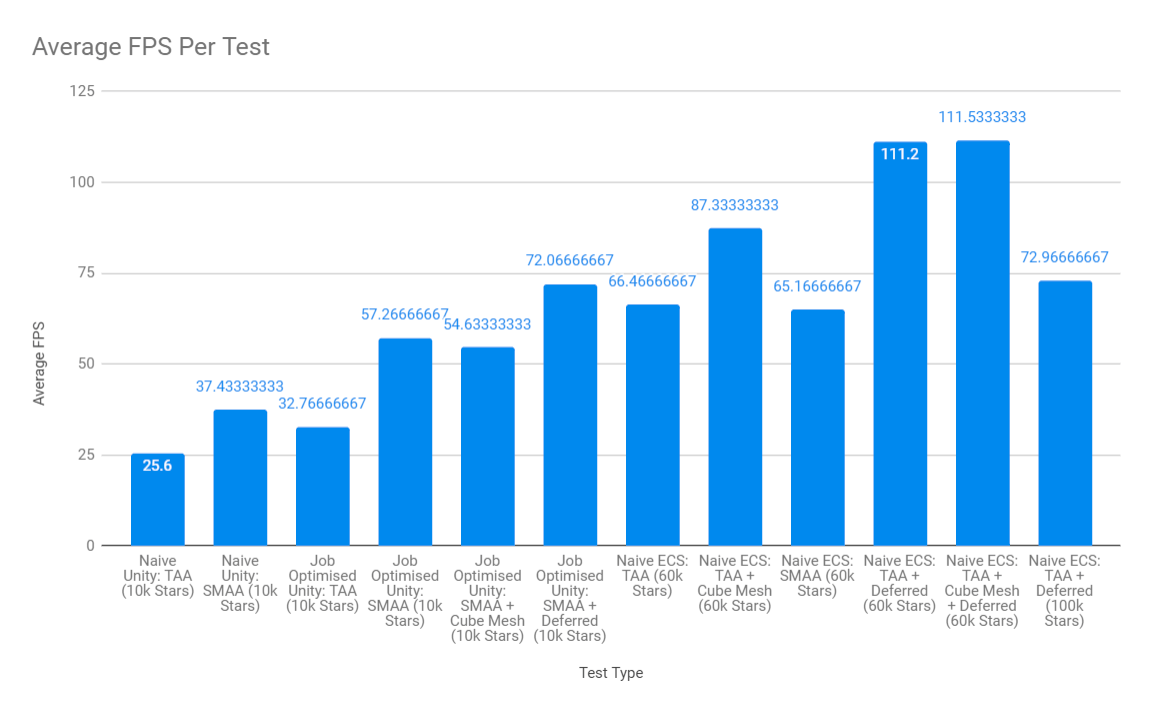
\includegraphics[width=1\textwidth]{Figures/averageFpsPerTest.png}
    \caption[Average Framerate Per Test]{The average framerate for all tests}
    \label{fig:averageFPS}
\end{figure}

Frames per second (shortened to FPS or framerate) is a performance metric that is very commonly seen in games. It works well for aggregating the overall performance of all the tests so they can be presented in one bar chart. The average framerates for these tests are calculated by taking the total amount of recorded frames and dividing them by 30 as this was the recording period in seconds. The average framerate for all the tests can be seen in Figure~\ref{fig:averageFPS}. 

In general, if we take galaxy size differences into account, making use of Unity ECS resulted in the best performance. The best performing test in the Job Optimised Unity condition sees similar performance to one of the ECS tests although the latter consists of ten times as many stars and a more complex anti-aliasing algorithm. 